
%(BEGIN_QUESTION)
% Copyright 2015, Tony R. Kuphaldt, released under the Creative Commons Attribution License (v 1.0)
% This means you may do almost anything with this work of mine, so long as you give me proper credit

\noindent

\vskip 5pt


\textbf{Introdusjon}

I denne oppgaven skal du justere og kalibrere utstyr for måling av trykk tre DP-celler og en trykkbryter. 

\begin{itemize}[noitemsep]
	\item Rosemount 3051 \href{https://www.emerson.com/documents/automation/reference-manual-rosemount-3051-pressure-transmitter-hart-r-protocol-en-89452.pdf}{manual}
	\item Rosemount Model E1151 Analog DP-celle
	\item Fuji Eletric FCX-AII serie transmitter \href {https://www.instrumart.com/assets/Fuji-FCX-manual.pdf}{manual}
	\item Danfoss RT200 trykkbryter \href{https://assets.danfoss.com/documents/149203/AN17908643810101-000501.pdf}{manual}
\end{itemize}


For Fjui Eletric transmitteren skal du tilpasse transmitteren til montering i ulike posisjoner(se manaul), såkalt zero calibration. For resten av transmitterne skal du justere og kalibrere for oppgitte LRV og URV(disse får du av lærer når du starter oppdraget)

$$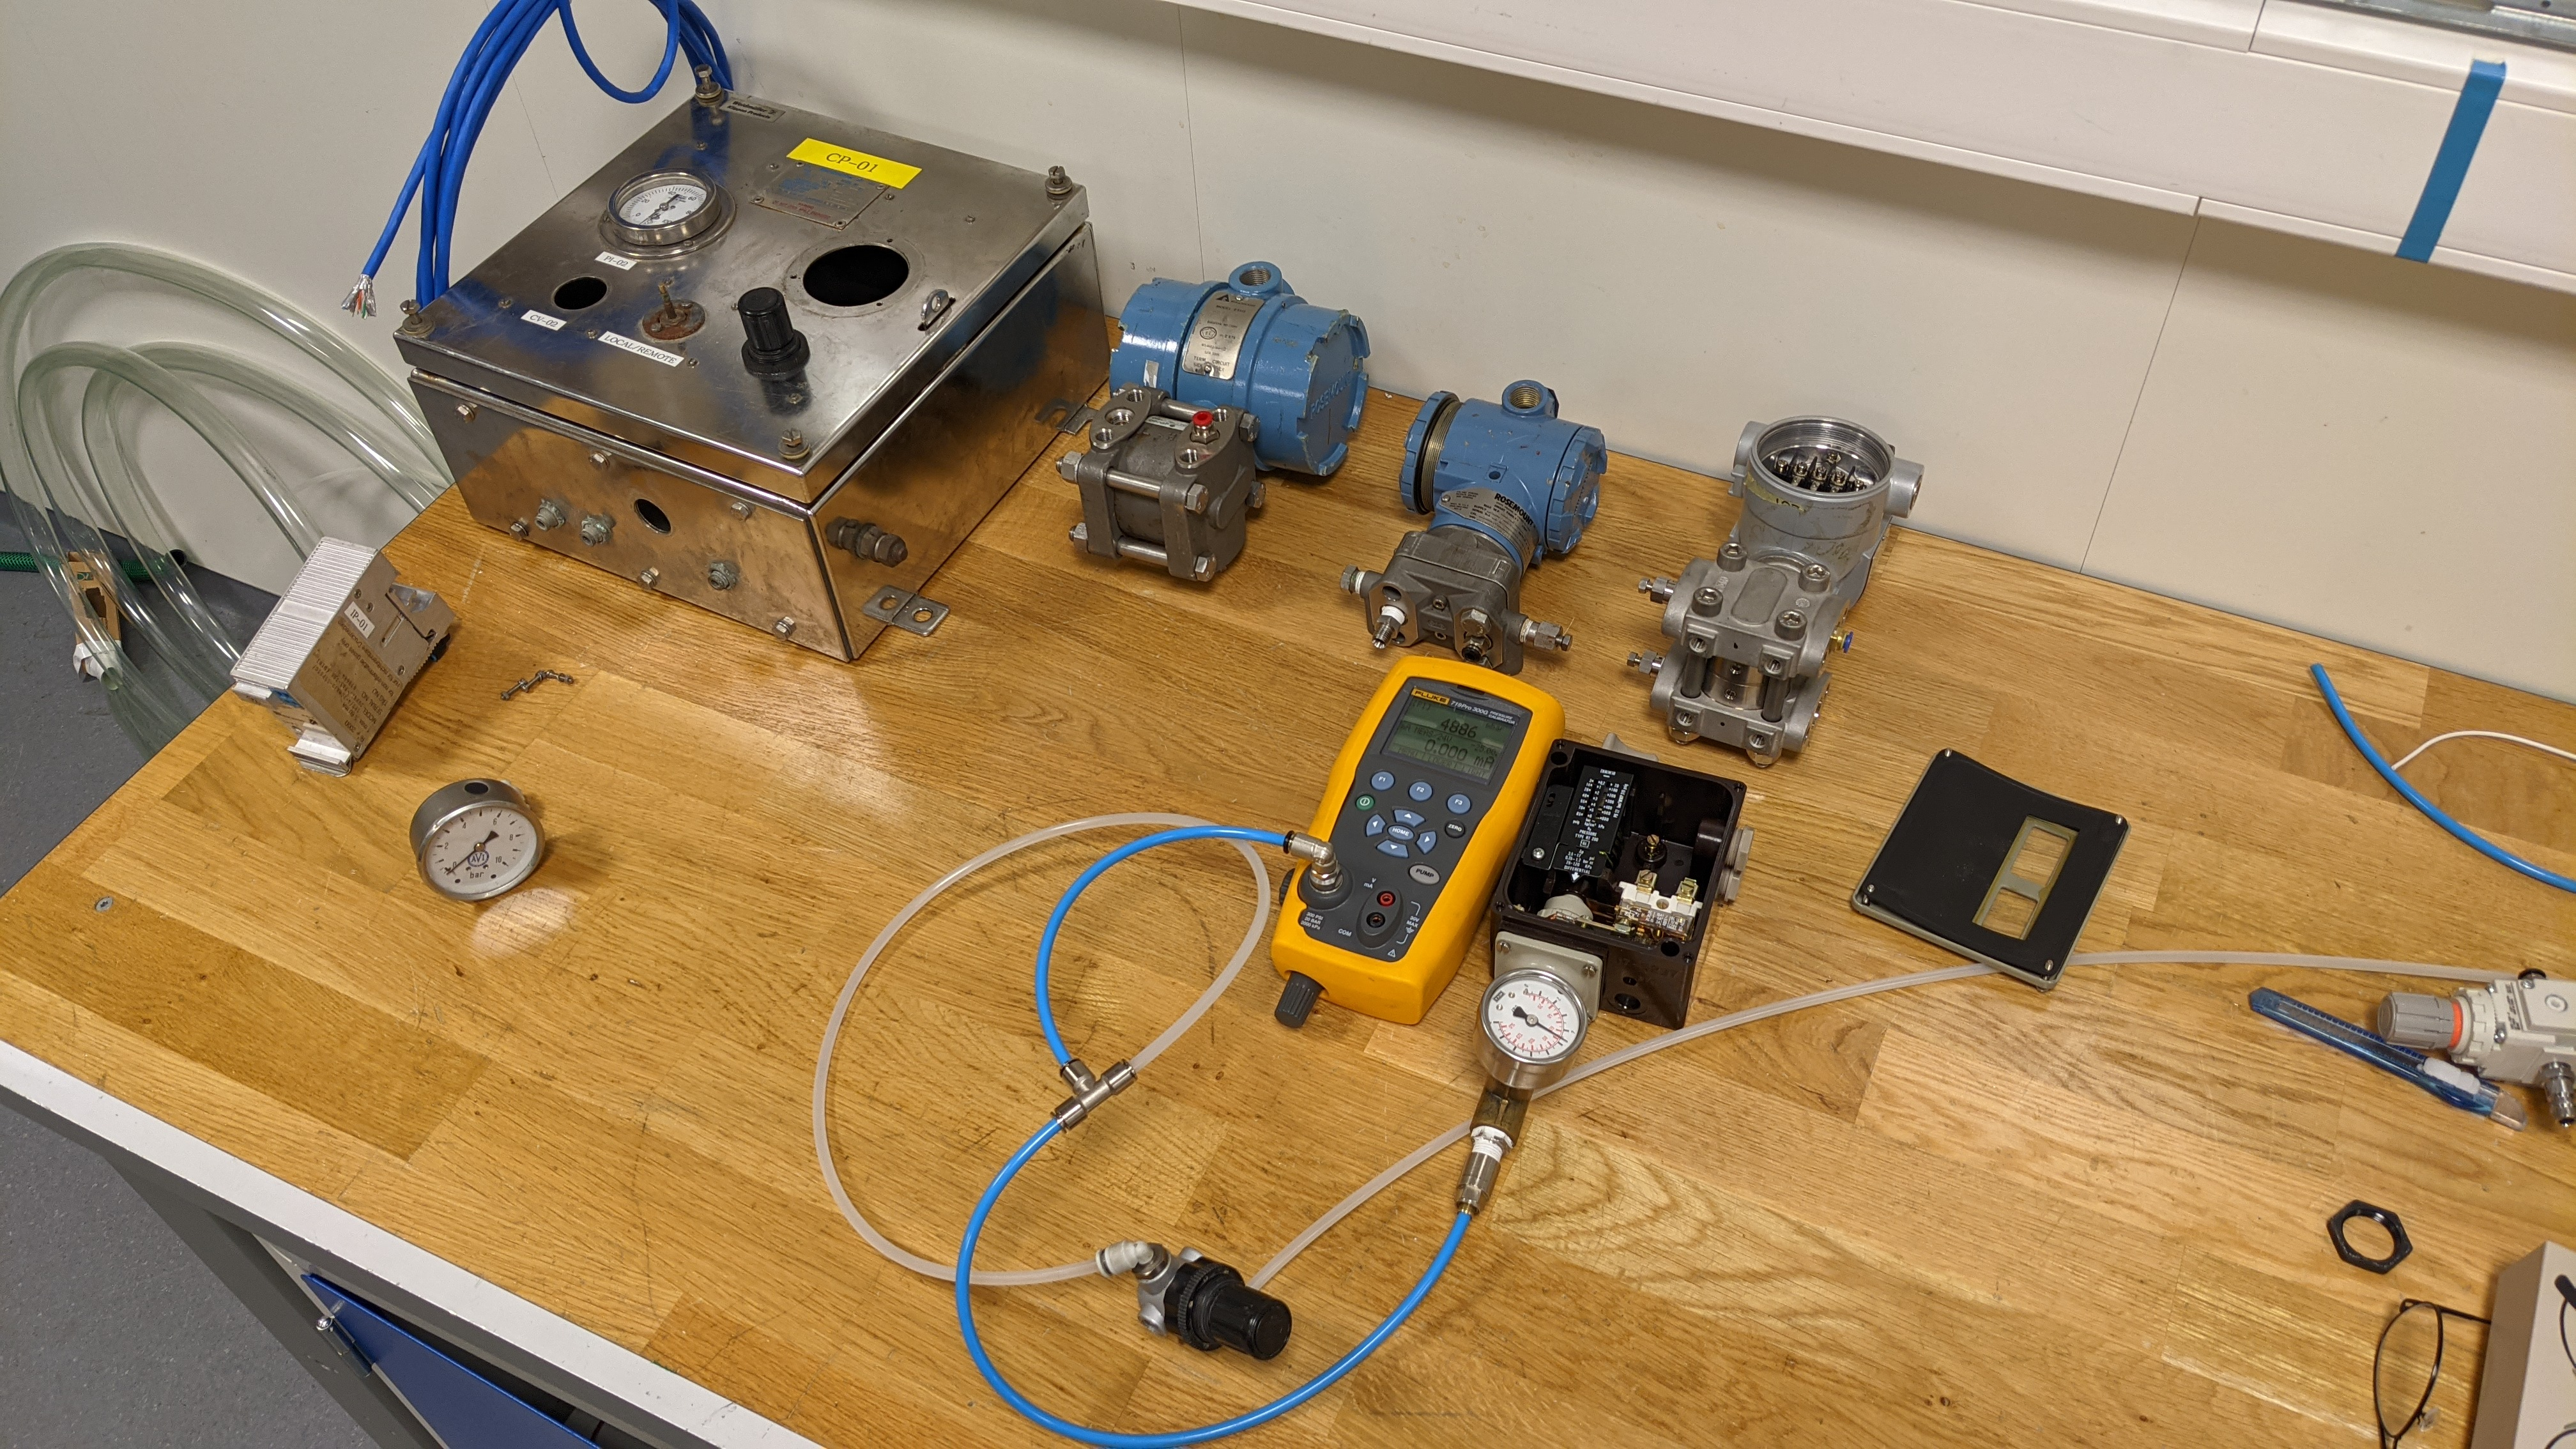
\includegraphics[width=13cm]{i04842x01.jpg}$$\\


\textbf{Arbidsoppdrag -- teorioppgaver}

\begin{enumerate}
	\item Les vedlagt bruksanvisning for å sette dere inn i virkemåten til utstyret.
\end{enumerate}
\textbf{Arbidsoppdrag -- planlegging}
Eksempel og en verktøysliste for danfoss trykkbryteren kan være følgende:

\vskip 5pt 
\begin{itemize}[noitemsep]
	\item Trykkbryter danfoss
	\item trykkregulator og manometer
	\item multimeter
\end{itemize}

Følgende punkter kan være med med i en fremdriftsplan:

Oppgaver\begin{enumerate}
	\item Utføre en As found kalibrering 
	\item Justere inn til nye LRV og URV
	\item Utfør en As left kalibrering 
	\item lagre dokumentasjon for jobben.
\end{enumerate}
\textbf{Arbidsoppdrag -- gjennomføring}

\textbf{Arbidsoppdrag -- dokumentasjon}

\begin{enumerate}
	\item Beskriv hvordan du planla, gjennomførte og dokumentere jobben. Forklar hvordan en slik pressostat kan nyttes til en pumpe eller kompressor. Forklar eventuelle avvik dere måtte observere under forsøket. 
\end{enumerate}




\noindent

\underbar{file i04842}
\vfil \eject
%(END_QUESTION)





%(BEGIN_ANSWER)


%(END_ANSWER)





%(BEGIN_NOTES)


%INDEX% Arbeisdoppdrag, Målesystemer, Nivå 1, Stasjon10, Kalibrering, Trykkbryter

%(END_NOTES)


